
\documentclass{Dissertate}

\usepackage{multirow}
\usepackage{todonotes}
\usepackage{graphicx}            
\usepackage{booktabs}
\usepackage{tcolorbox}
\tcbuselibrary{most}
\hyphenpenalty=100

\begin{document}
\chapter*{\centering Cognitive Abstractions for \\ Visual Communication}

\qauthor{\centering Kushin Mukherjee}
{\centering \large \textbf{Dissertation Proposal } \par}

\vspace{2mm}

%%%%%%%%%%%%%%%%%%%%%%%
% Projects: 

% FYP++
% Semantic Spaces
% Color GPT

% THINGS Drawings
% SEVA
% Semantic Disc Theory


% Neural Loci

%%%%%%%%%%%%%%%%%%%%%%%
Visual communication is a fundamental cornerstone of modern human endeavors.
The most ornate and staggering of buildings begin as strokes on paper shared between architects, Nobel prize-worthy scientific advances begin as graphs shared among lab members, and the most ineffable of emotions can be communicated with a single patch of color.
These examples speak to the ability of the human mind to abstract away from the naturalistic world and distill visual features in order to pithily create new visual artifacts that convey complex ideas.
How does the mind generalize from concrete prior experiences to produce and understand visual abstractions -- sketches, charts, maps, and diagrams?

This dissertation and my research program more generally investigates the representations and the operations on those representations that facilitate our ability to produce and understand visual abstractions.
I argue that these representations are necessarily \textit{cross-modal}, reflecting the rich patterns of covariation not only in the visual world but between vision and natural language. 
I also argue that the manner in which we deploy these representations for visual communication are context sensitive requiring good cognitive models to `decode' behavior from the representations.
Lastly, I evaluate progress in artificial intelligence, driven by deep neural network models of vision and language, using a host of evaluations across several studies, each of which touch upon visual abstraction in different ways.
I support these arguments using a suite of studies focused on two domains of cognition -- color semantics and drawing.

In the following pages, I present chapter summaries along with notes on the present status of the studies in each chapter. The chapters on experimental studies are broadly organized into two parts. Part 1 covers studies that characterize and measure abstract visual representations.
Part 2 focuses on studies that describe how such representations support visual communication behavior and how these behaviors themselves might be a window into the nature of these representations.
Briefly, the dissertation will be structure as follows —
\begin{enumerate}
    \item \textbf{Introduction}. This chapter presents the problem of visual abstraction and provides an overarching background and brief review of relevant work in the cognitive sciences.
    \item \textbf{Chapter 1: Characterizing an abstract semantic space for
color-concept associations}. This chapter presents a model for how color-concept associations are represented in the mind in a \textit{color semantic space}. I evaluate this model and show that it can estimate color-concept associations for unseen colors and concepts.
\item \textbf{Chapter 2: Characterizing the representational basis of visual similarity for line drawings}. Using triplet similarity judgements, studies in this chapter show that people's perceived similarity of simple line drawings and shapes is not perfectly captured by deep neural network models of vision, which fail to represent the cognitive factors that organize perceived similarity.
\item \textbf{Chapter 3: How do we communicate using colors?}. Here, I present \textit{semantic discriminability theory}, which outlines the conditions for being able to create visual encoding systems that are interpretable.
The theory is presented in the context of color semantics, where I show how it is possible to create color encoding systems for both abstract and concrete concepts alike.
\item \textbf{Chapter 4: How do we communicate using drawings?}. This chapter covers a series of production-recognition experiments using drawings that highlight the flexibility and chart the limits of humans' and machines' ability to convey object concepts using strokes.

\item \textbf{Chapter 5: Neural loci for visual abstractions}. This final experimental chapter outlines a study for delineating the neural locus of color-concept associations, which constitutes a critical step towards reconciling notions of visual abstraction with established literature on visual processing in the human brain.
\item \textbf{Conclusion.} The closing chapter will summarize the findings from across the preceding chapters and will propose a path towards future progress in visual abstraction.


\end{enumerate}







\section*{\textbf{Introduction}}

The goal of this opening chapter is twofold -- (1) to equip the reader with adequate background on the key behavioral phenomena explored in the studies that constitute this dissertation and (2) to situate the problem of visual abstraction within the larger canon of visual and semantic cognition.
The brief review presented will motivate the argument that visual communication is highly flexible and that humans utilize visually abstract features to communicate  concepts that range from abstract to concrete.
It will also recall how semantic representations have been characterized in cognitive science, with an emphasis on the importance of cross-modality.
Lastly, it will provide a primer on modern models of vision and semantics generally insofar as they are treated as scientific models in the context of this document, which are evaluated against human behavior.

\begin{tcolorbox}[
    colback=gray!10,  % background color (light gray)
    colframe=black!50, % frame color (darker gray)
    arc=4mm,         % corner radius
    boxrule=2pt      % frame thickness
]
Much of this section will involve synthesizing across different projects and unifying them under the theme of abstractions for visual communication. 
Materials from both my breadth and depth prelim can be partially used to inform parts of the introduction, but the majority of this will be new. 
I hope to dedicate short sections of this introduction to establish relevant background in areas that might not be represented in this thesis (e.g., cross-cultural and non-human primate work).
\end{tcolorbox}


\section*{\textbf{Part 1: Representations for visual abstraction}}
\section*{Chapter 1: Characterizing an abstract semantic space for \\ color-concept associations  }

People show systematic associations between colors and concepts when probed using a variety of color-concept judgement tasks.
How is it the case that people show such associations for even abstract concepts that lack visual features?
We show, by measuring people's associations between 71 colors representative of perceptual color space and 70 diverse concepts, that people's color-concept associations are low-rank and can be efficiently represented using a set of interpretable dimensions.
These dimensions constitute a \textit{color semantic space}.
By estimating the position of any concept or color in this space, we show that we are able to estimate associations between any color-concept pair.
We additionally show that the structure of this space cannot be explained by natural language processing (NLP) vectors, highlighting the limitation of purely linguistic representations and the importance of perceptual input in shaping color-concept associations.

We also evaluate modern multimodal models like GPT-4o in their ability to estimate color-concept associations when probed in similar ways to how humans are. 
We find patterns of associations while still distinct from that of humans, still approaches human-levels of consistency matching alternative modeling approaches.
These results are taken as a proof-of-concept of how assocations between perceptual properties and abstract concepts can be learned from data at scale with a powerful enough learning model.

\begin{figure}[htpb!]
    \centering
    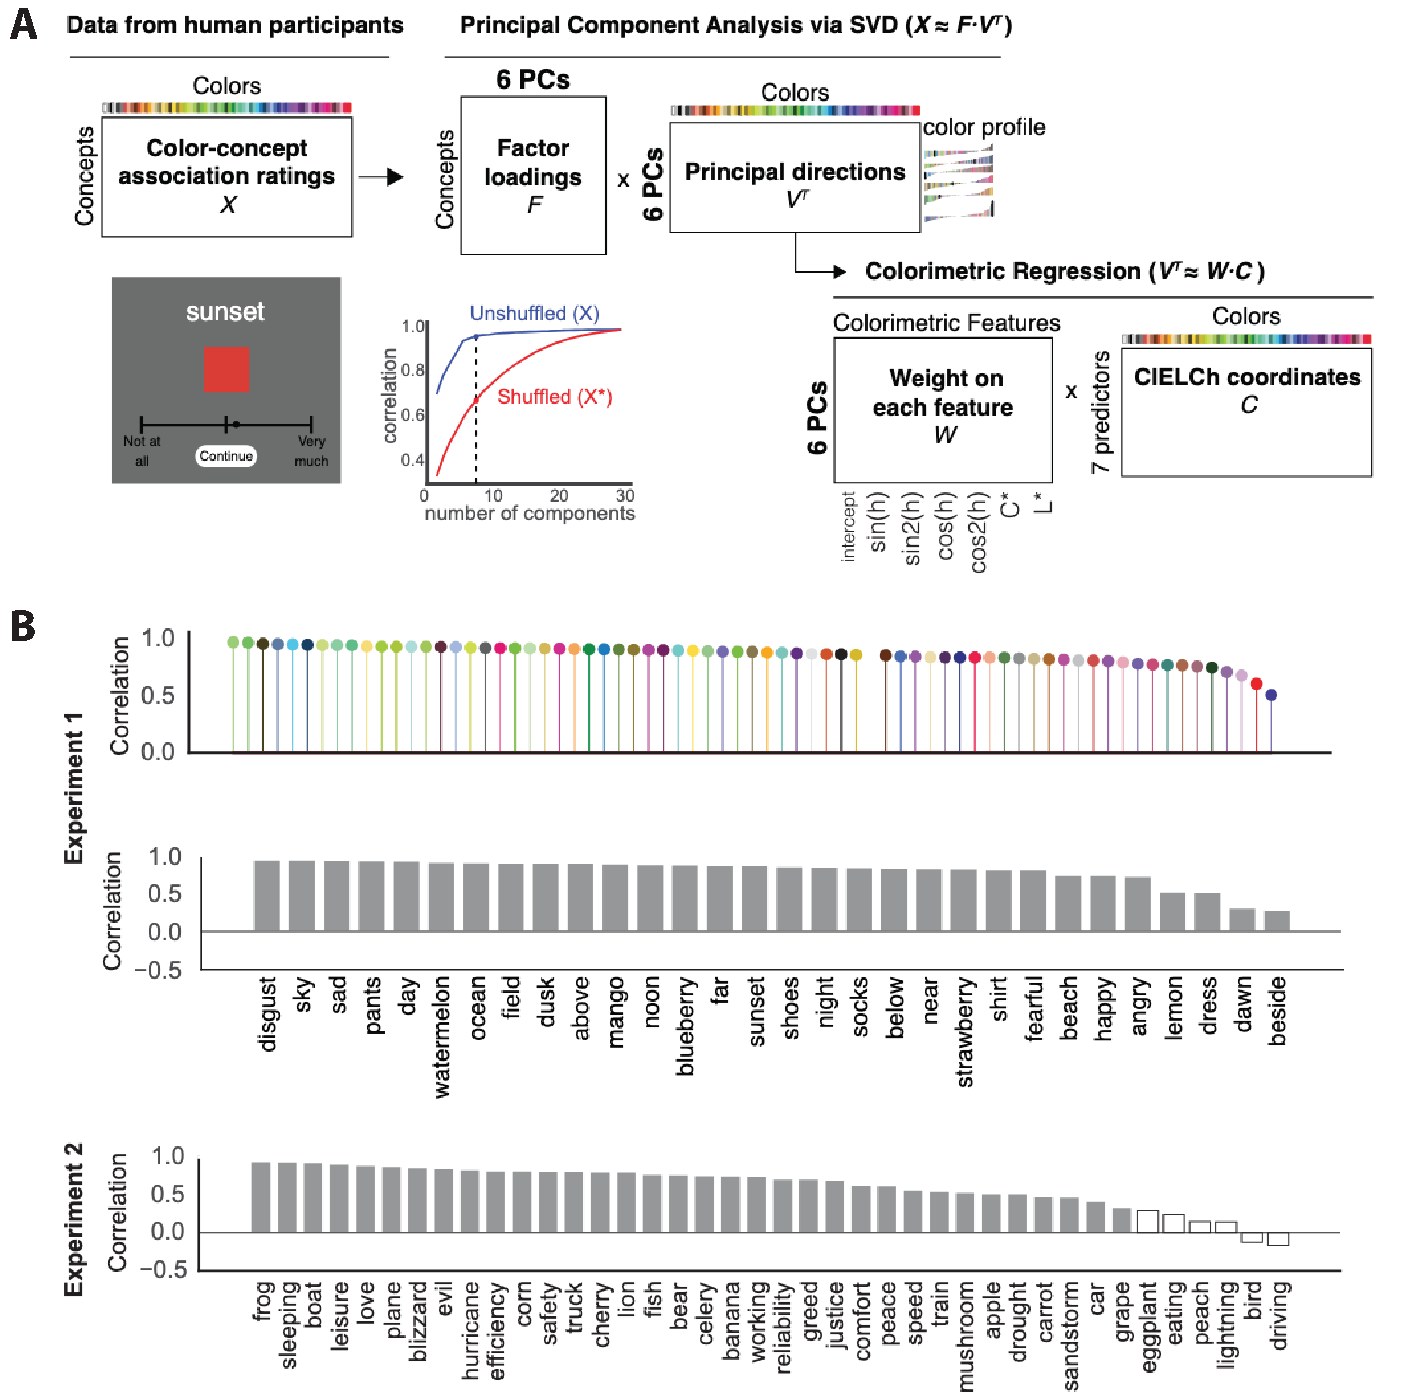
\includegraphics[width=.8\linewidth]{proposal/figures/chap1.pdf}
    \caption{(A) Our model for representing color semantic space by applying dimensionality reduction techniques on matrices of color-concept association rating judgements and using colorimetric regression models to characterize the dimensions of the space. (B) Correlations between true ratings and predicted ratings using our model for new colors and concepts. Overall, the model is effective for most colors and concepts.}
    \label{fig:chap1}
\end{figure}

\begin{figure}[htpb!]
    \centering
    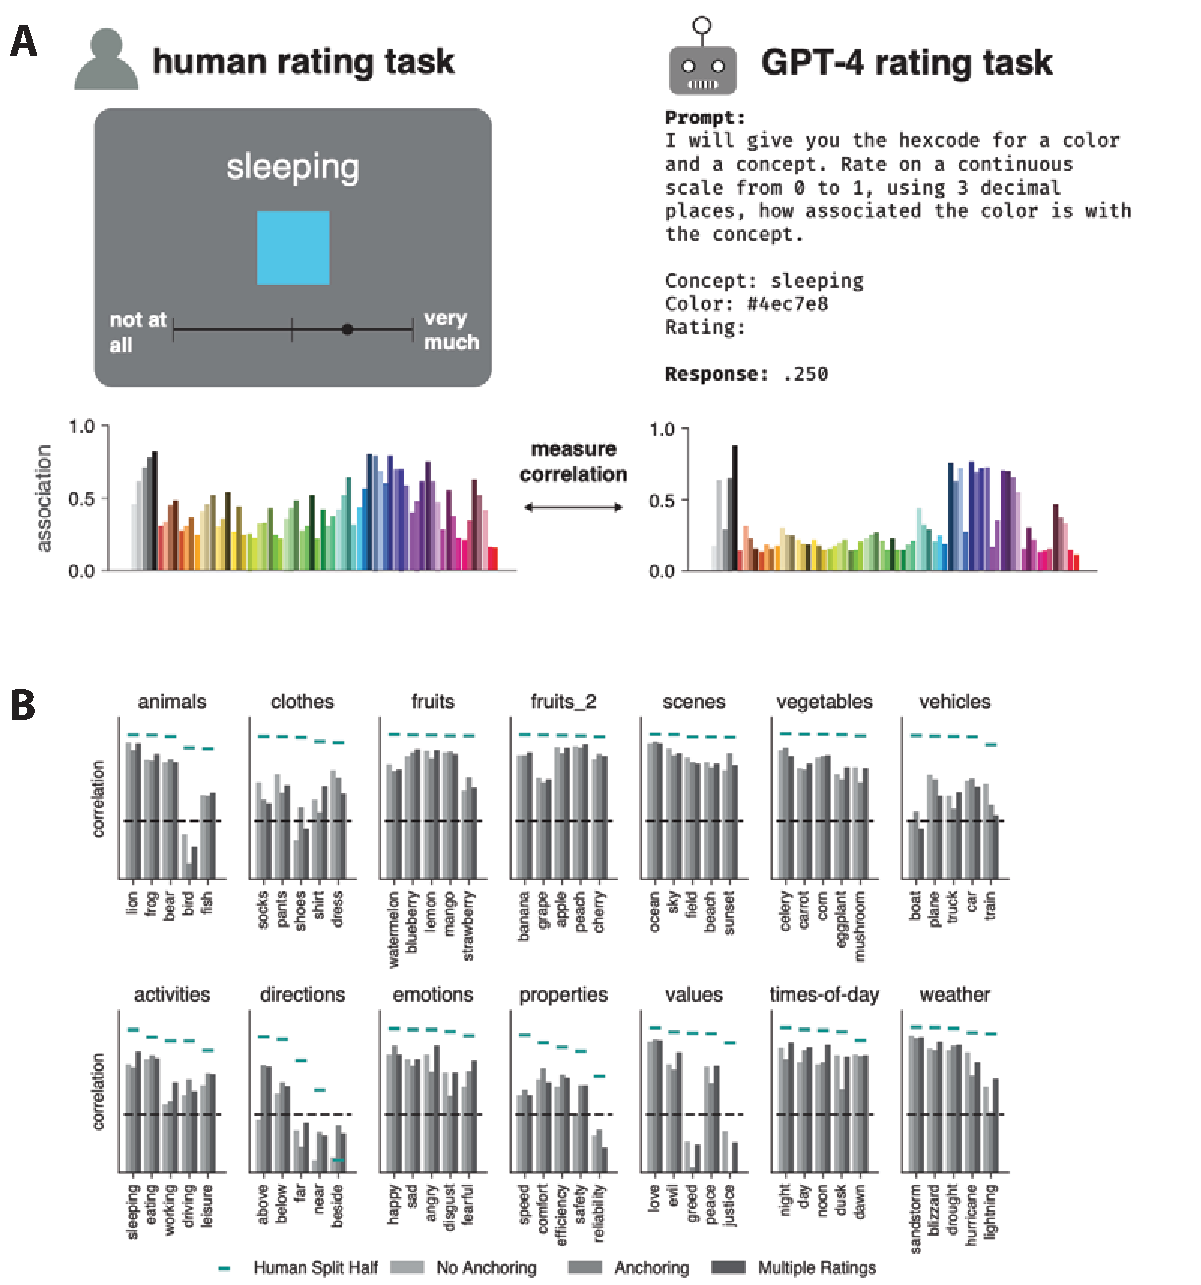
\includegraphics[width=.8\linewidth]{proposal/figures/chap1b.pdf}
    \caption{(A) Human and LLM testing paradigms for collecting color-concept association ratings. (B) Corelation between true ratings and GPT-4 ratings for a variety of abstract and concrete concepts. GPT-4 fails to reach human levels of consistency but is as effective of competing approaches. }
    \label{fig:chap1b}
\end{figure}

\begin{tcolorbox}[
    colback=gray!10,  % background color (light gray)
    colframe=black!50, % frame color (darker gray)
    arc=4mm,         % corner radius
    boxrule=2pt      % frame thickness
]
Contents for this chapter have been presented at VSS 2021 and 2022. All the data for this chapter has been collected, results have been written up, and the manuscript (Mukherjee, Lessard, Gleicher, Schloss, \& Rogers, in prep) is near ready for submission.
The goal is to submit the manuscript this semester.
\end{tcolorbox}

\section*{Chapter 2: Characterizing the representational basis of visual similarity \\ for line drawings}

Humans are able to discern the difference and similarity between both real world objects and abstract renderings of them, such as in line drawings.
Children can also do this effortlessly when presented with abstract renderings that do not conform to the natural world. 
What is the representational basis for these judgements? 
One possibility is that these judgements are based on visual properties of the images alone.
An alternative is that highly semanticized representations support similarity judgements between visual artifacts that are abstract versions of real-world referents.
We first measure people's perceived similarity for a dataset of densely annotated drawings using a triplet judgement task.
We set low-dimensional embeddings of each item based on the triplet judgements as a target and evaluate the ability of representations derived from deep neural networks (DNN) of vision and simple cognitive and perceptual factors to decode this structure.
We find that while both low level visual properties of drawings (such as spatial frequency and shape) help explain the structure, the majority of variance is explained by the semantic category of drawings.
Additionally, DNN features cannot decode the target similarity structure without the help of these other factors.
The best performing DNN models were found to be models trained to represent the similarity structure between images and text (CLIP), supporting the notion that cross-modal learning supports learning human-like visual representations.
\begin{figure}[htpb!]
    \centering
    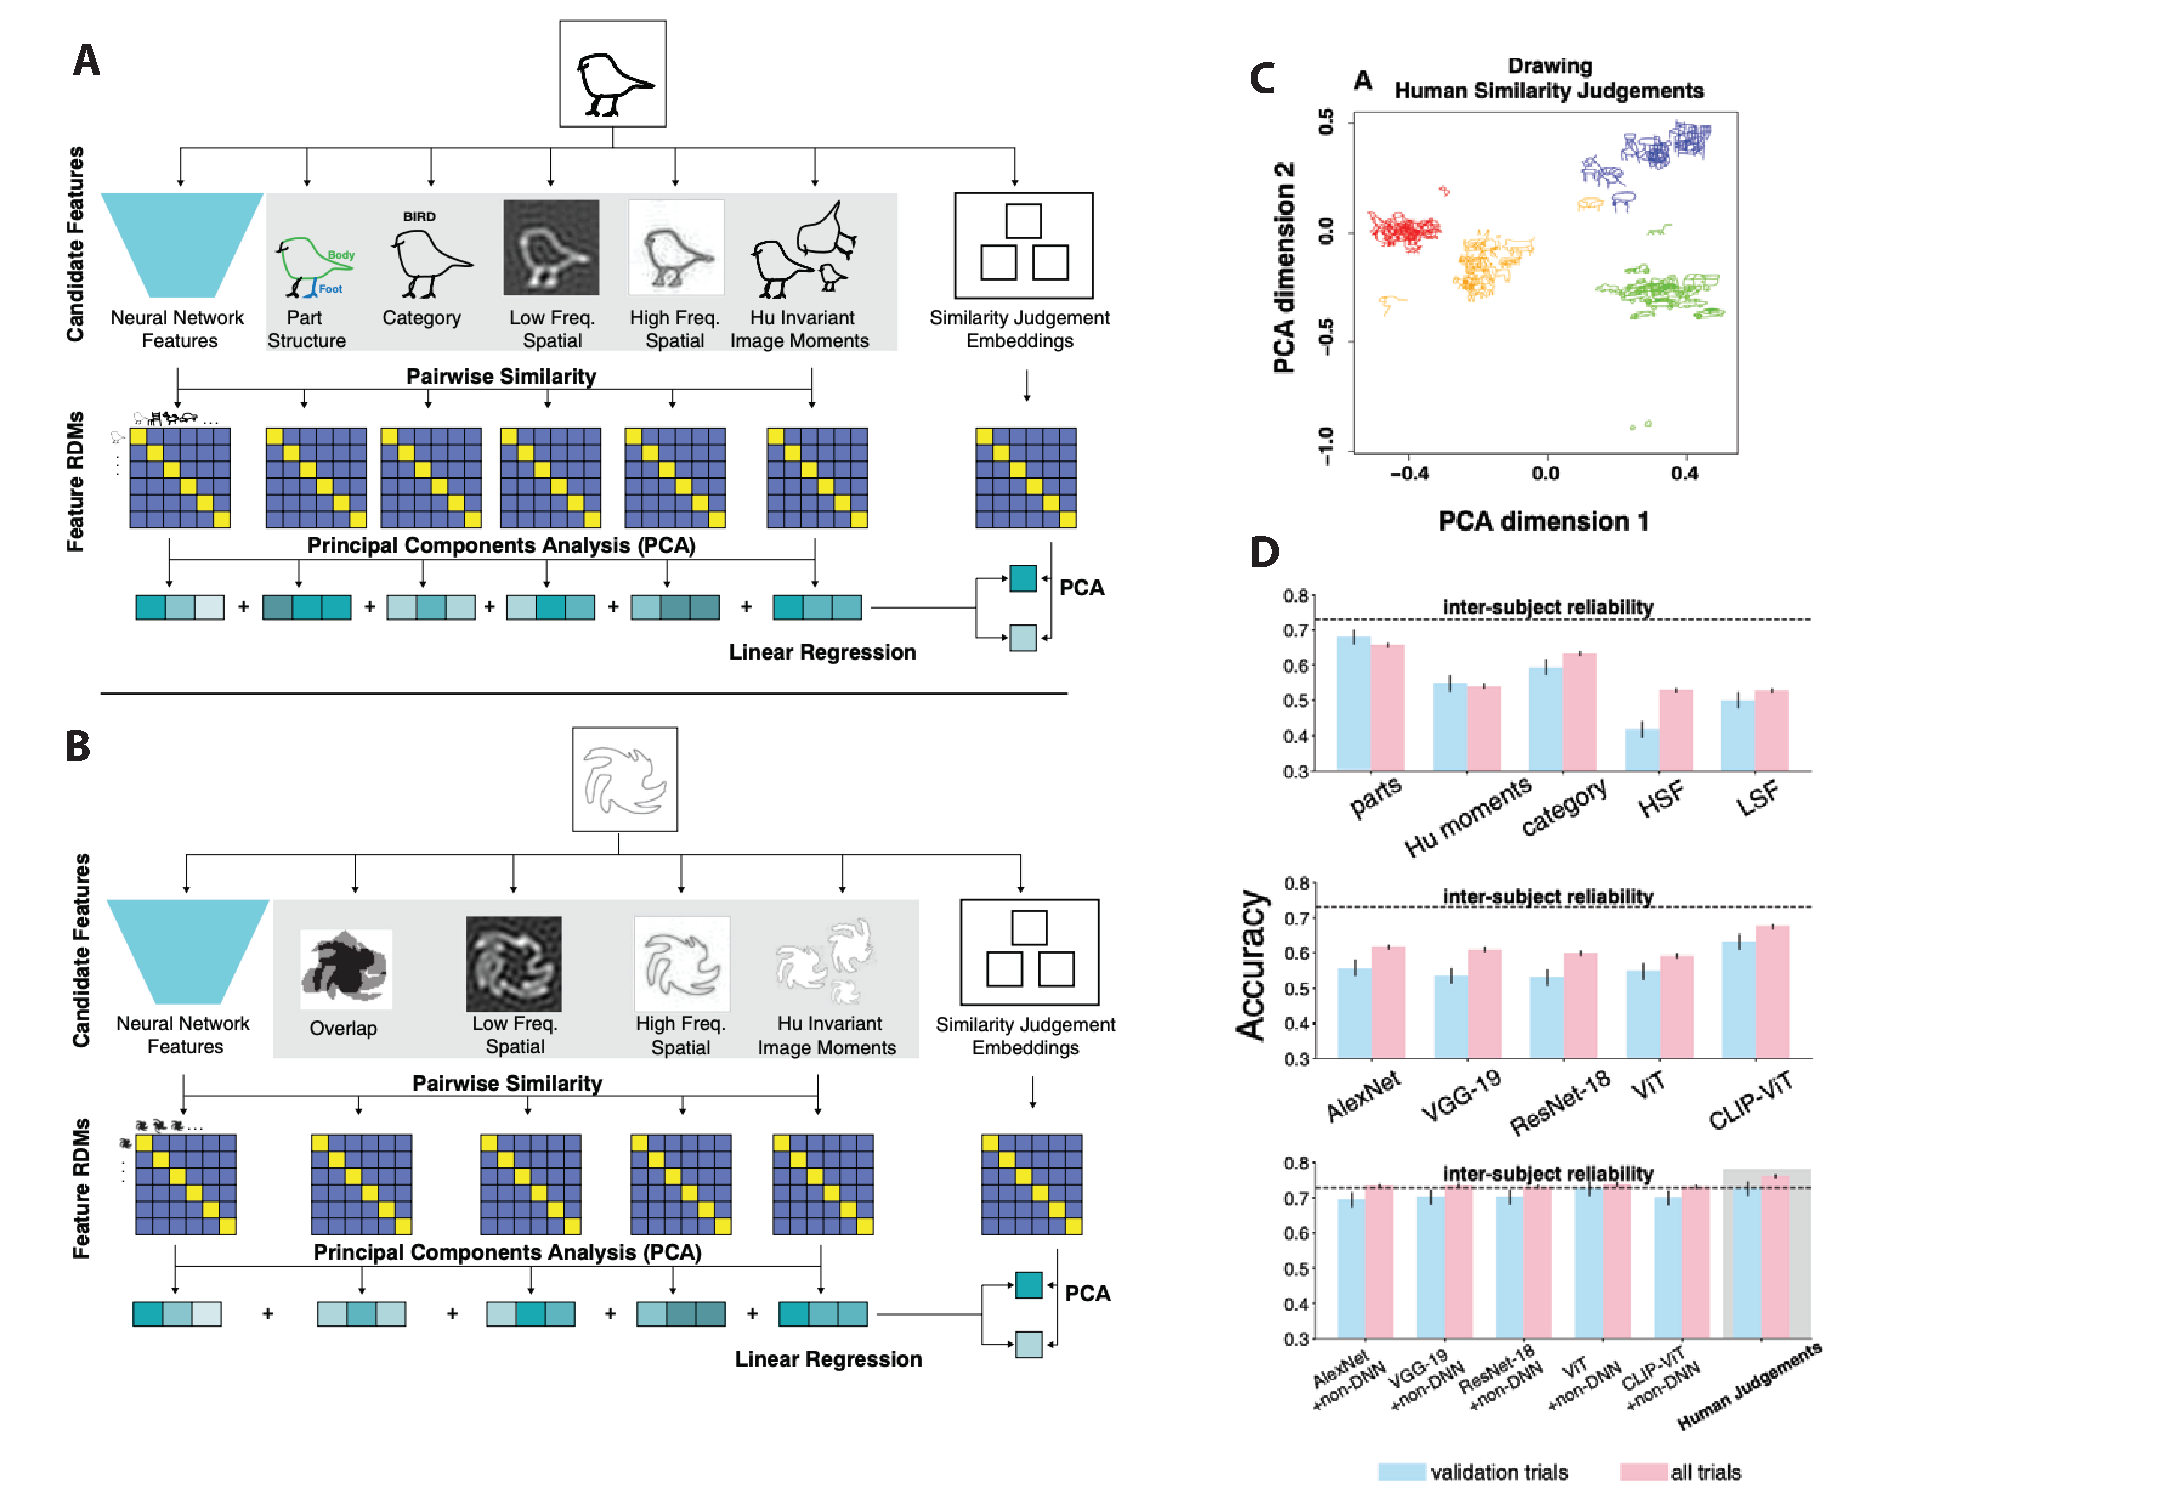
\includegraphics[width=.8\linewidth]{proposal/figures/chap2.pdf}
    \caption{Analysis schematic showing the DNN, perceptual and cognitive features used to predict human similarity judgements in (A) line drawings of objects and (B) simple shape contours. (C) coordinates of drawings of each category (bird, car, chair, dog) after performing dimension reduction on the embeddings derived from triplet similarity judgements. (D) The ability of perceptual and cognitive features (top), vision models (bottom), and joint models combining vision model and cognitive/perceptual representations (bottom) in predicting human similarity judgements. Only when DNN features are combined with our hypothesized factors do models accurately predict human ratings.  } 
    \label{fig:chap2}
\end{figure}



\begin{tcolorbox}[
    colback=gray!10,  % background color (light gray)
    colframe=black!50, % frame color (darker gray)
    arc=4mm,         % corner radius
    boxrule=2pt      % frame thickness
]
Contents for this chapter are based on my first year project (FYP) and has also been presented at VSS 2020.
Experiment 2, which estimated similarity structures between `non-semantic' contour drawings, the inclusion of CLIP as a key vision model and several analyses for both Experiments 1 and 2 were added after the FYP defense.
The manuscript (Mukherjee \& Rogers, 2024) was accepted and published in \textit{Memory \& Cognition} in 2024.
\end{tcolorbox}


\section*{\textbf{Part 2: Leveraging abstractions for visual communication}}

\section*{Chapter 3: How do we communicate using colors?}

People’s associations between colors and concepts influence their ability to interpret the meanings of colors in information visualizations such as charts.
To the extent that stable associations exist between colors and concepts as outlined in earlier chapters, can we communicate about abstract concepts using color?
We showed that we indeed can, challenging earlier notions that some concepts are not `colorable' and cannot be conveyed using colors. We present a general framework for understanding the conditions determining when people can infer meaning from perceptual features using color as a key case study. This framework is referred to as \textit{semantic discriminability theory} and formally outlines the conditions that support communication using perceptual properties.
Specifically, the difference in the distributions of color associations between concepts help constrain which colors can be used as valid `messengers' of meaning.

Our theory of semantic discriminabilty rests on a model of how people's associations can lead to specific inferred assignments between colors and concepts in a visualization.
This chapter constitutes a key example of how abstract representations, here associations between perceptual properties and concepts, support and shape fundamentally important visual communication behavior -- chart comprehension.


\begin{figure}[htpb!]
    \centering
    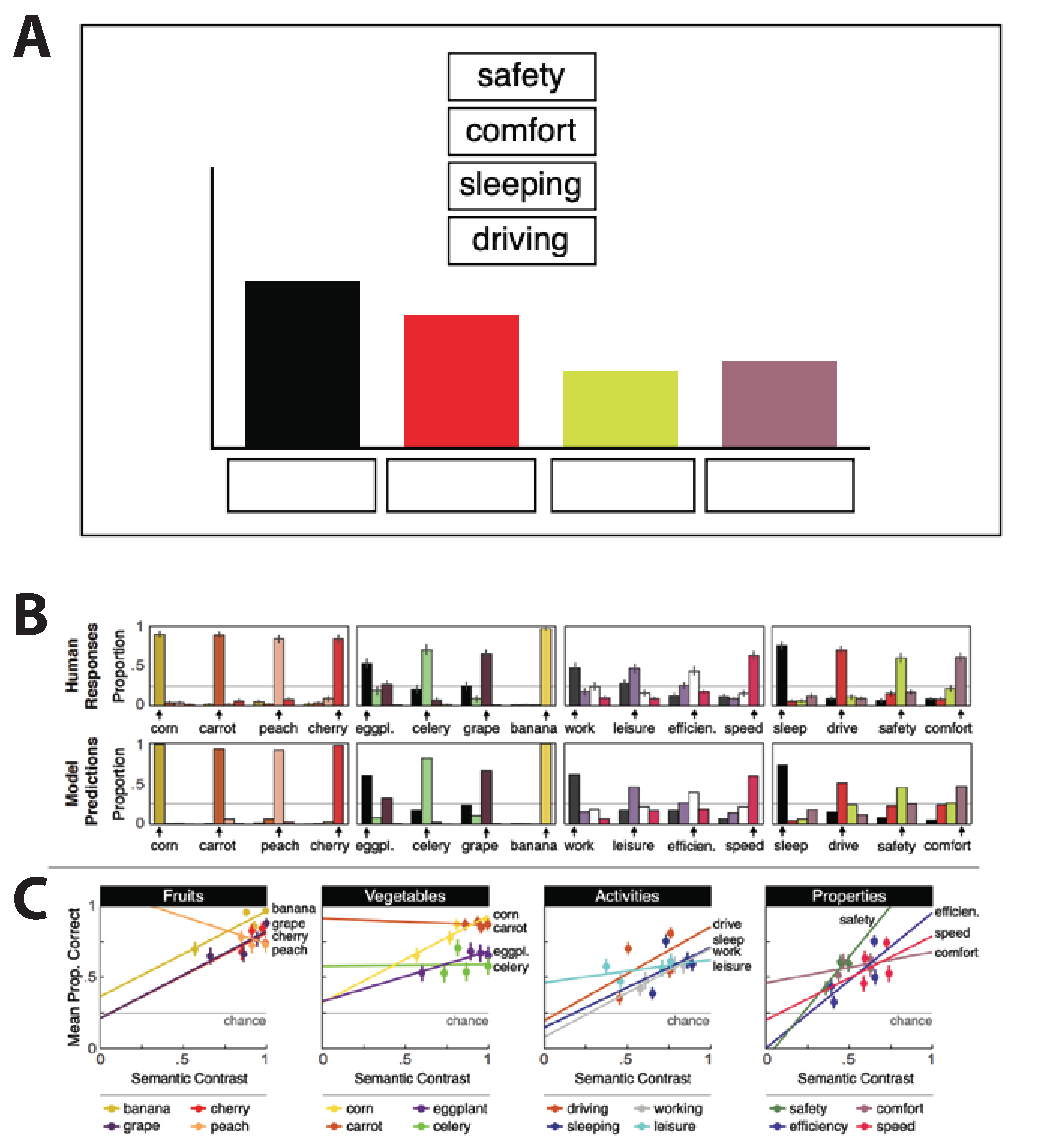
\includegraphics[width=.8\linewidth]{proposal/figures/chap3.pdf}
    \caption{(A) The task from Mukherjee et al. (2021). Participants had to choose which bar to assign each concept to. (B) Human patterns of color-to-concept mapping for palettes that vary in semantic discriminability and the ability of our models to predict those patterns. (C) Both abstract and concrete concepts can be easy or hard to communicate using colors depending on the set of concepts and colors in scope. }
    \label{fig:chap3}
\end{figure}




\begin{tcolorbox}[
    colback=gray!10,  % background color (light gray)
    colframe=black!50, % frame color (darker gray)
    arc=4mm,         % corner radius
    boxrule=2pt      % frame thickness
]
Contents for this chapter are based on Mukherjee, Yin, Sherman, Lessard \& Schloss (2021) and was published and presented at \textit{IEEE VIS}.
\end{tcolorbox}

\section*{Chapter 4: How do we communicate using drawings?}

The ability to use our visuosemantic representations of concept to both produce and recognize highly sparse line drawings is a particularly salient example of visual abstraction.
However drawings themselves can be made at many different levels of abstraction, from detailed to sketchy, and of any real-world concept.
This chapter emphasizes the importance of measuring drawing production and recognition at different levels of abstraction and for a representatively large variety of visual concepts in making progress towards a cognitive theory of visual abstraction.
It also highlights the role of drawing as a key behavior in better characterizing visual concepts.

The first set of studies vary the level of detail object drawings are depicted in by limiting the amount of time sketchers have during production.
We showed that while sparser drawings are harder to recognize \textit{correctly}, they are often labeled using semantic neighbors (e.g., a drawing of a dog might be labeled using `fox' or `cow') showing the robustness of people's visual abstractions.
Through fine-grained benchmarking of DNN models of both sketch production and comprehension, we characterize large outstanding gaps between even the most performant models and human behavior.
Here too we find that multimodal models fare the best.

The second set of studies extends the production-recognition paradigm to a large set of 1,854 object concepts.
A key finding is that there is wide concept-to-concept variability in their ability to be conveyed using drawings.
A key challenge for a general theory of visual abstraction will be to explain the conditions that constrain drawing-based communication similar to semantic discriminability theory.


\begin{figure}[htpb!]
    \centering
    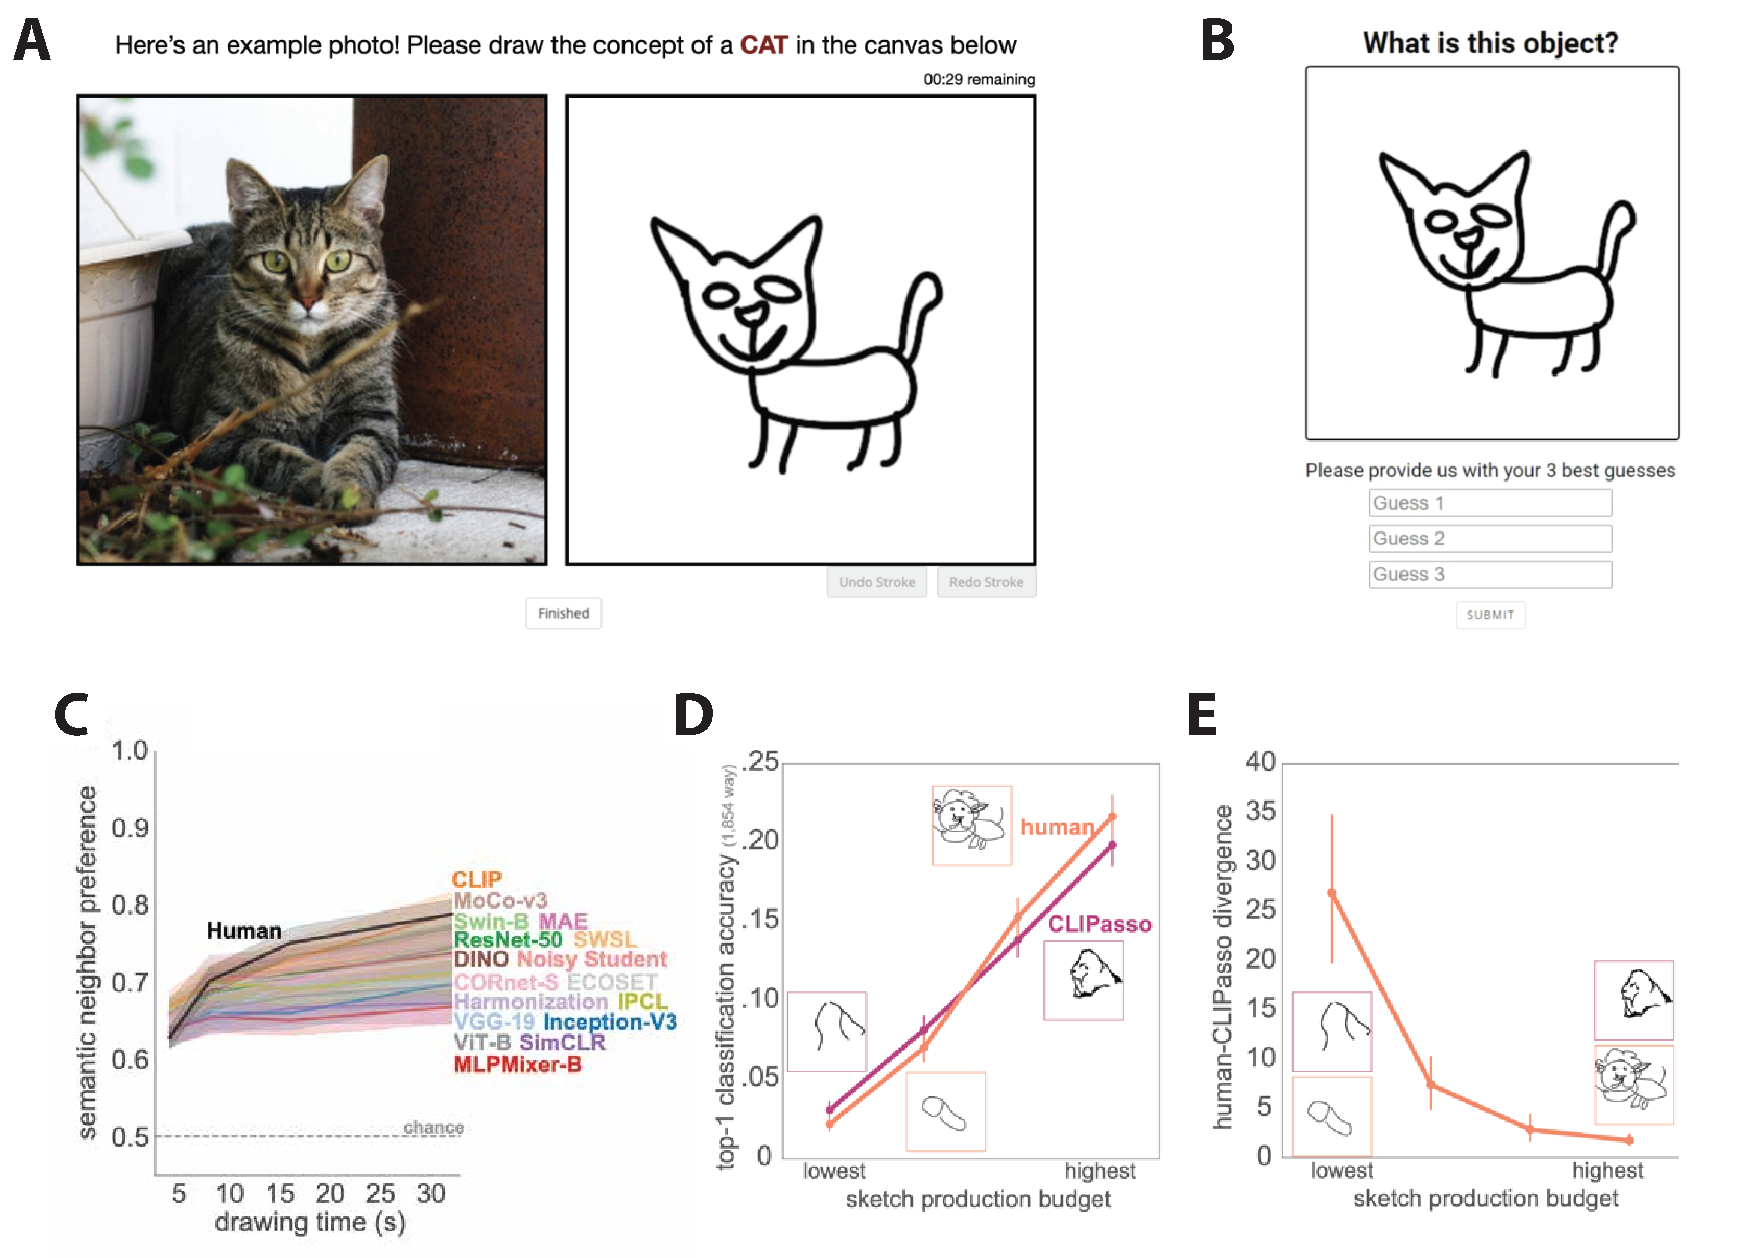
\includegraphics[width=.8\linewidth]{proposal/figures/chap4.pdf}
    \caption{(A) Interface for drawing production task from Mukherjee et al. (2023). (B) Interface for the drawing recognition task from Mukherjee et al. (2023). (C) The likelihood of drawings being labeled as close semantic neighbors as a function of different abstraction levels (drawing time) in humans and vision models. (D) How accurately humans label drawings made by other humans or a CLIP-based sketcher model (CLIPasso) at different abstraction levels. How similar are the labels produced by human guessers when looking at human vs. machine made drawings. While both human-made and machine-made drawings are recognized at about the same rate across abstraction levels, the specific labels that are applied to them become more divergent the most abstract the drawing.}
    \label{fig:chap4}
\end{figure}


\begin{figure}[htpb!]
    \centering
    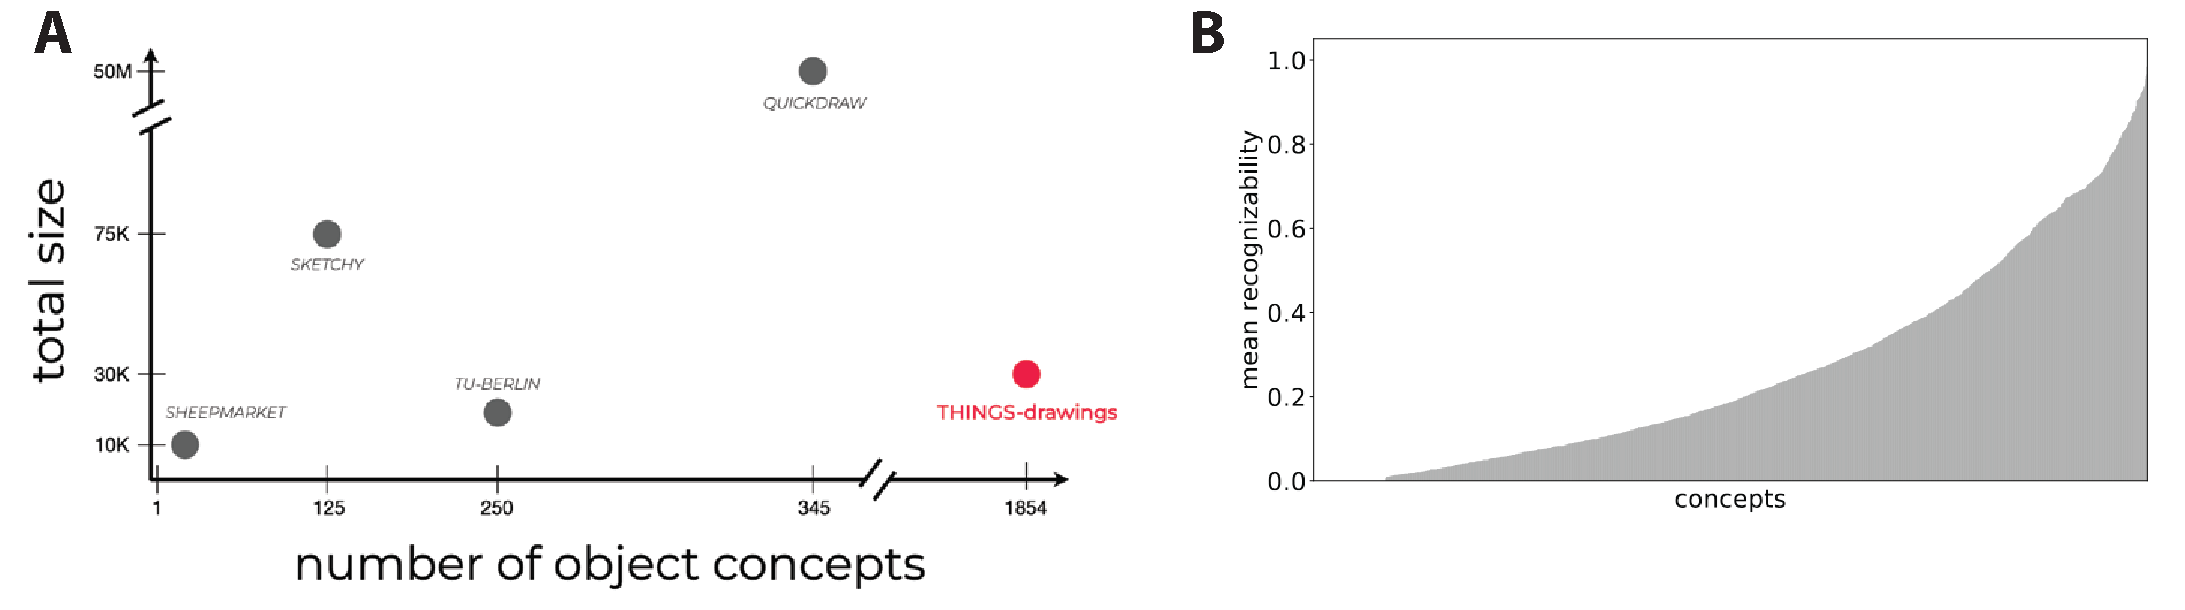
\includegraphics[width=.8\linewidth]{proposal/figures/chap4b.pdf}
    \caption{(A) Our new drawing dataset in terms of its total number of drawings and semantic diversity relative to existing datasets. (B) Variability in recognizability of different concepts. The x-axis is each of the 1,854 concepts in the THINGS dataset, the y-axis is how often drawings of that concept are labeled using the label that was shown to the sketcher when asked to draw it.}
    \label{fig:chap4b}
\end{figure}



\begin{tcolorbox}[
    colback=gray!10,  % background color (light gray)
    colframe=black!50, % frame color (darker gray)
    arc=4mm,         % corner radius
    boxrule=2pt      % frame thickness
]
Contents for this chapter are based on two cross-university collaborative projects that I have led. 
The manuscript (Mukherjee, Huey, Lu, Vinker, Shamir, \& Fan, 2023) reflecting the first set of experiments have been written up and published at \textit{NeurIPS}.
Data for the second set of experiments has been collected and the results are mostly written up in manuscript form (Mukherjee, Huey, Hebart, Fan, \& Bainbridge, in prep).
The goal is to submit the latter manuscript this semester.
\end{tcolorbox}



\section*{\textbf{Part 3: Neural loci for visual abstractions}}

What is the neural basis for visual abstraction? 
Before building neural computational models that support the range of behaviors described thus far, a primary question concerns \textit{where} these representations might lie in the human brain.
Is there a highly localist seat of visual abstraction or is the neural code highly distributed reflected the hypothesized cross-modal nature of the representations that support the phenomenon.
The last set of experiments will focus in once more on the color-concept associations described in chapters 1 and 3 and aim to estimate the neural loci of these associations.
We will estimate color-color and color-concept associations by using a 2 alternative forced-choice task paradigm where people will be asked to choose which of two color patches or two concepts is most similar to a target color patch.
The hypothesis is that the first variant of the task will allow us to decode representations that support purely perceptual similiarty among colors while the second will allow decoding more abstract and cross-modal representations.
Using recent statistical tools for decoding distributed neural signals, I hope to show where these representations might lie and whether they are highly concentrated in one cortical region or whether there are measurably distinct, distributed codes across individuals.


\section*{Chapter 5: Where are visual abstractions housed in the brain?}

\begin{tcolorbox}[
    colback=gray!10,  % background color (light gray)
    colframe=black!50, % frame color (darker gray)
    arc=4mm,         % corner radius
    boxrule=2pt      % frame thickness
]
This chapter will be based on experiments that as of now have yet to be conducted.
There exists a sketch of the experimental design for the behavioral task that participants will be asked to complete in the scanner. 
The aim is to pilot the behavioral task online and finalize the pipeline for the neural data collection and preprocessing this semester.
Early in the new year, the aim is to begin neural data collection and conduct the relevant analyses.
\end{tcolorbox}


\section*{Conclusion}

Each of the studies covered in this dissertation tackle distinct behaviors, across distinct domains, in human versus artificial minds.
However, the findings all speak to the nature of abstract visual representations and how they might be structured and deployed in visual communication generally.
Understanding how we learn to represent and produce visual abstractions has implications for a host of behaviors beyond the ones covered here, which span reasoning, learning, and communication.
Having stronger cognitive theories of visual abstraction will allow us to also better use it as a key benchmarking target in the evolving landscape of artificial intelligence models.

In this closing chapter, I will synthesize the findings from each chapter and lay out what a general cognitive theory of visual abstraction might look like and how it might lead to progress in fields beyond psychology including artificial intelligence and education.

% \clearpage
% \bibliography{proposal/proposal}
% \addcontentsline{toc}{chapter}{References}
\bibliographystyle{apacite}

% %!TEX root = ../dissertation.tex
\newpage

% If you do want an image in the colophon:
\begin{figure}
  \vspace{20pt}
  \centering
  \hspace*{-32pt}
  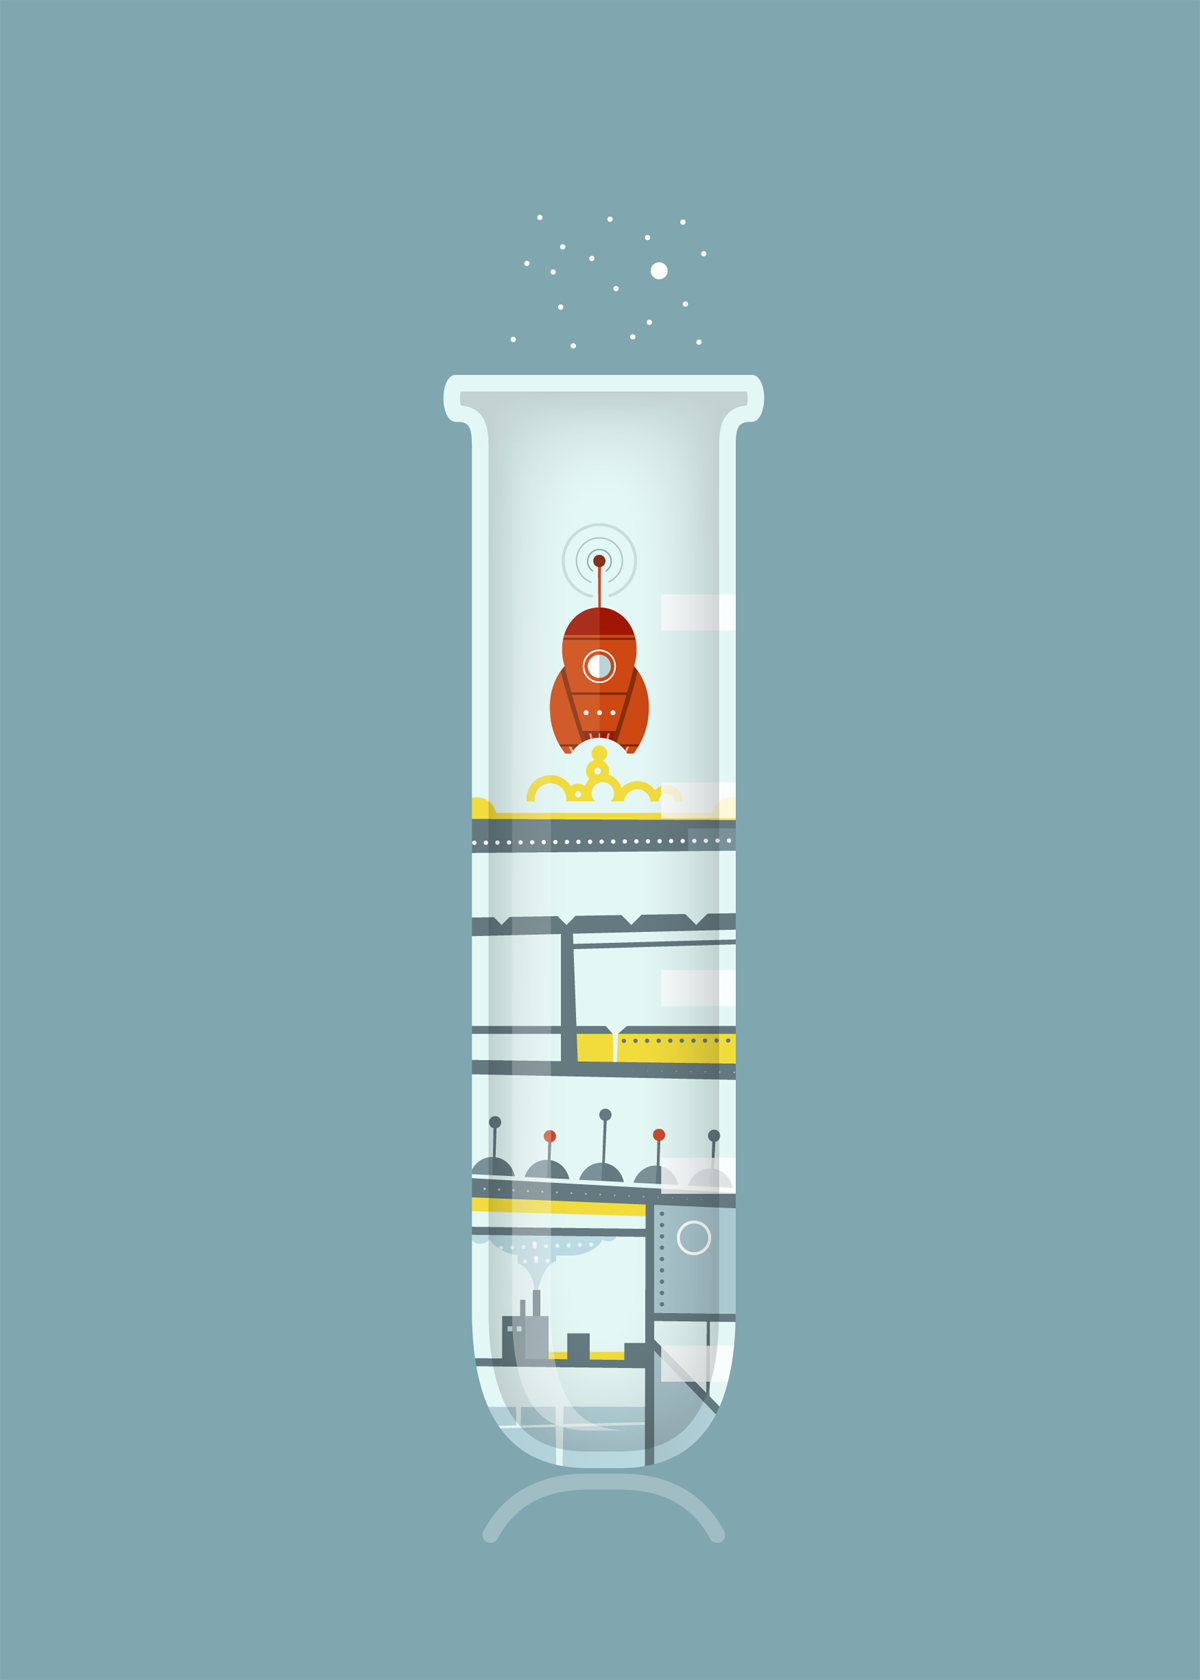
\includegraphics[width=0.42\textwidth]{endmatter/colophon.png}
\end{figure}

% If you don't want an image in the colophon:
% \vspace*{200pt}

\begin{center}
\parbox{200pt}{\lettrine[lines=3,slope=-2pt,nindent=-4pt]{\textcolor{SchoolColor}{T}}{his thesis was typeset} using \LaTeX, originally developed by Leslie Lamport and based on Donald Knuth's \TeX. The body text is set in 11 point Egenolff-Berner Garamond, a revival of Claude Garamont's humanist typeface. The above illustration, \textit{Science Experiment 02}, was created by Ben Schlitter and released under \href{http://creativecommons.org/licenses/by-nc-nd/3.0/}{\textsc{cc by-nc-nd 3.0}}. A template that can be used to format a PhD dissertation with this look \textit{\&} feel has been released under the permissive \textsc{agpl} license, and can be found online at \href{https://github.com/suchow/Dissertate}{github.com/suchow/Dissertate} or from its lead author, Jordan Suchow, at \href{mailto:suchow@post.harvard.edu}{suchow@post.harvard.edu}.}
\end{center}


\end{document}
